\chapter{CROCODDYL - LAAS-CNRS}\label{chapter1}
\section{Introduction}
\subsection{Motivation}
Crocoddyl is an \textbf{optimal control library for robot control under contact sequence}. Its solver is based on an efficient Differential Dynamic Programming (DDP) algorithm. Crocoddyl computes optimal trajectories along with optimal feedback gains. It uses Pinocchio for fast computation of robot dynamics and its analytical derivatives \cite{crocoddylweb}. 

Crocoddyl is focused on multi-contact optimal control problem (MCOP) which has the form:

$$\mathbf{X}^*,\mathbf{U}^*=
\begin{Bmatrix} \mathbf{x}^*_0,\cdots,\mathbf{x}^*_N \\
				  \mathbf{u}^*_0,\cdots,\mathbf{u}^*_N
\end{Bmatrix} =
\arg\min_{\mathbf{X},\mathbf{U}} \sum_{k=1}^N \int_{t_k}^{t_k+\Delta t} l(\mathbf{x},\mathbf{u})dt$$
subject to
$$ \mathbf{\dot{x}} = \mathbf{f}(\mathbf{x},\mathbf{u}),$$
$$ \mathbf{x}\in\mathcal{X}, \mathbf{u}\in\mathcal{U}, \boldsymbol{\lambda}\in\mathcal{K}.$$
where
\begin{itemize}
\item the state $\mathbf{x}=(\mathbf{q},\mathbf{v})$ lies in a manifold, e.g. Lie manifold $\mathbf{q}\in SE(3)\times \mathbb{R}^{n_j}$, $n_j$ being the number of degrees of freedom of the robot.
\item the system has underactuacted dynamics, i.e. $\mathbf{u}=(\mathbf{0},\boldsymbol{\tau})$,
\item $\mathcal{X}$, $\mathcal{U}$ are the state and control admissible sets, and
\item $\mathcal{K}$ represents the contact constraints.
\end{itemize}

Note that $\boldsymbol{\lambda}=\mathbf{g}(\mathbf{x},\mathbf{u})$ denotes the contact force, and is dependent on the state and control.

\subsection{Features}
According to the description in the Github repository \cite{crocoddylweb}, it comprises the following features:

Crocoddyl is \textbf{versatible}:
\begin{itemize}
\item various optimal control solvers (DDP, FDDP, BoxDDP, etc) - single and multi-shooting methods
\item analytical and sparse derivatives via Pinocchio
\item Euclidian and non-Euclidian geometry friendly via Pinocchio
\item handle autonomous and nonautomous dynamical systems
\item numerical differentiation support
\end{itemize}

Crocoddyl is \textbf{efficient} and \textbf{flexible}:
\begin{itemize}
\item cache friendly,
\item multi-thread friendly
\item Python bindings (including models and solvers abstractions)
\item C++ 98/11/14/17/20 compliant
\item extensively tested
\end{itemize}



\section{How-To}
\subsection{Install}
\subsubsection{Two ways to go}
Basically there are existing two ways of installing Crocoddyl: 
\begin{itemize}
\item Option 1: Installation via the \textit{robotpkg } package manager
\item Option 2: Installation from source
\end{itemize} 
I personally would recommend the installation through \textit{robotpkg}, since it preserves you from dealing with the multiple dependencies of Crocoddyl and therefore seems to be the faster approach. Generally you should decide beforehand which python version you want to use. This effects the robotpkg version as well as the export of the PYTHONPATH variable. 

\subsubsection{Installation via robotpkg (preferred)}
Steps for installing via robotpkg according to the installation section of \cite{crocoddylweb}
\begin{enumerate}
	\item Add robotpkg as source repository to apt:
	\begin{verbatim}
	sudo tee /etc/apt/sources.list.d/robotpkg.list <<EOF
	deb [arch=amd64] http://robotpkg.openrobots.org/wip/packages/debian/pub $(lsb_release -sc) robotpkg
	deb [arch=amd64] http://robotpkg.openrobots.org/packages/debian/pub $(lsb_release -sc) robotpkg
	EOF
	\end{verbatim}
	\item Register the authentication certificate of robotpkg:
	\begin{verbatim}
	curl http://robotpkg.openrobots.org/packages/debian/robotpkg.key | sudo apt-key add -
	\end{verbatim}
	\item You need to run at least once apt update to fetch the package descriptions:
	\begin{verbatim}
	sudo apt-get update
	\end{verbatim}
	\item The installation of Crocoddyl:
	\begin{verbatim}
	sudo apt install robotpkg-py27-crocoddyl # for Python 2
	sudo apt install robotpkg-py36-crocoddyl # for Python 3
	\end{verbatim}
	\item Finally you will need to configure your environment variables (watch out for the python version!), e.g.:
	\begin{verbatim}
	export PATH=/opt/openrobots/bin:$PATH
	export PKG_CONFIG_PATH=/opt/openrobots/lib/pkgconfig:$PKG_CONFIG_PATH
	export LD_LIBRARY_PATH=/opt/openrobots/lib:$LD_LIBRARY_PATH
	export PYTHONPATH=/opt/openrobots/lib/python3.6/site-packages:$PYTHONPATH
	\end{verbatim}
\end{enumerate}

\subsubsection{(Installation from source)}
If you prefer installing Crocoddyl from source, the following steps should do the work:
\begin{verbatim}
git clone https://github.com/loco-3d/crocoddyl.git 
git submodule update --init
mkdir build && cd build
export PKG_CONFIG_PATH=/opt/openrobots/lib/pkgconfig
cmake -DCMAKE_INSTALL_PREFIX=/opt/openrobots  ..
make
sudo make install
\end{verbatim}
Additionally you will have to install the dependent libraries (i.e. pinocchio, example-robot-data (optional for examples, install Python loaders), gepetto-viewer-corba (optional for display), jupyter (optional for notebooks) and matplotlib (optional for examples) and fix the incude paths.

\subsection{Running the Examples}
Since the installation through robotpkg did not provide you with the examples from the git repository, you should clone the repo \cite{crocoddylweb} for getting the data. You do not have to build the library, since it already is installed. 
In the cloned repository go to \textit{/examples}. For running e.g. the bipedal walking example, just type
\begin{verbatim}
python3 bipedal_walk.py
\end{verbatim}
and you will see the calculations for optimal gait trajectories running in the console. 
You propably want to view your results now. For displaying the results, we need to install the gepetto-viewer:
\begin{verbatim}
 sudo apt install robotpkg-py36-qt4-gepetto-viewer-corba
\end{verbatim}
The examples provide a \textit{plot} and \textit{display} argument. In order to display the 3D results and also plot some data, just do 
\begin{verbatim}
gepetto-gui
\end{verbatim}
for starting the 3D environment and then, in another terminal
\begin{verbatim}
python3 bipedal_walk.py display plot
\end{verbatim}



\section{Abstract Workflow}
For each node (i.e. each timestep) of the optimal control problem, 
\begin{enumerate}
\item Load robot data (URDF, SRDF, Meshes)
\item Define Action Models (Dynamics+Costs) for running and terminal states 
	\begin{itemize}
	\item Setup a cost model
	\item Add the desired cost functions (state, control, frame-placement etc.)
	\item Calculate Integrated \& Differential Action Model (IAM/DAM) based on the model
	\end{itemize}
\item Define the optimal control problem (knots+IAMs, initPose)
\item Solve the Shooting Problem
\end{enumerate}



\section{Issues and Insights}
\subsection{Issues Encountered}
Since Crocoddyl currently is under active development, there frequently will occure smaller incompatibilities because of versioning issues.This is a brief overview of emerged difficulties:
\begin{itemize}
\item Python versioning errors in the examples. 

The examples most often are written for python2, which means that if you are under python3, you will have to adapt some commands (e.g. lists handling, matplotlib, print).
\item Crocoddyl versioning errors in the examples. 

Since Crocoddyl depends on other libraries (i.e. Pinnochio, example\_robot\_data), there sometimes occured errors with the class because they were not updated. 
\item Confusions displaying the results via the Gepetto-Viewer

The Gepetto-Viewer is used for displaying the robots and resulting trajectories from optimization. The examples only contain out of the box solutions. If one wants to simply display a robot in some specified pose (e.g. the initial pose) the following, quite unintuitive, commands have to be applied:
\begin{verbatim}
display = crocoddyl.GepettoDisplay(rh5_legs, 4, 4, frameNames=[rightFoot, leftFoot])
display.display(xs=[x0])
\end{verbatim}
\end{itemize}

\subsection{Cost Functions}
Notes:
\begin{itemize}
\item The cost function can contain multiple \textit{cost items} (i.e state/control error, frame displacements or center of mass tracking).
\item Weights are considered in the costs via scalar multiplication with the identity matrices (Ix, Ixx etc.) of the according cost item. 
\item These weighted matrices of cost items are simply summed up within a \textit{costModelContainer}.
\end{itemize}

\subsection{Joint Limits}
\begin{itemize}
\item Input Data: Within the URDF file, for each joint there are specified the
\begin{itemize}
	\item torque limit (effort),
	\item position limits (lower, upper),
	\item velocity limit.
\end{itemize}
\item These limits are not automatically taken into account in Crocoddyl when solving a shooting problem, but explicitly have to be adressed.
\item \textbf{Torque Limits}: Require the use of specific solvers, standard ddp is not sufficient. Implemented solvers that can handle torque limits explicitly are: 
\begin{itemize}
\item BoxDDP (Compare Tassa method \cite{tassa2014control})
\item BoxFDDP (Novel solver that is under development at LAAS)
\end{itemize}
\textbf{State Limits (Pos/Vel)}: Position and Velocity limits can be handled via penalization, i.e. added as cost terms to the optimization problem.  
\end{itemize}

\subsection{Introduction: Bipedal Walking in Crocoddyl}
\begin{itemize}
\item A long walk consists of multiple gaitphases, each phase is a single shooting problem.
\item These problems are generated with \textit{createWalkingProblem()} involving one left and one right foot step.
\item Each shooting problem contains various locomotion phases
	\begin{itemize}
	\item Double support at beginning (both legs on ground) via \textit{createSwingFootModel()}
	\item Right step (Swing-up and swing-down phase equally distributed) init via    	\textit{createFootstepModels()}
	\item Double support again
	\item Left step
	\end{itemize}	
\item In the end, all knots of all phases are basically one \textit{swingFootModel}. They only vary in the adressed foot, and if a CoM task or a swingFootTask is set.
\item The \textit{swingFootModel} is an IAM containing a 
	\begin{itemize}
	\item 6D multi-contact model,
	\item Cost model (CoM position tracking, contact friction cone, foot placement) and
	\item Differentiation (DAM) and Integration (IAM) routines.
	\end{itemize}
\end{itemize}

\subsection{Multi-Contact Model}
\subsubsection{Previous: Assume foot to have a point contact}
\begin{itemize}
\item Each \textit{swingFootModel}, meaning each knot of the OC, includes at least one individual contact model.
\item The number of contact models depends is specified via \textit{supportFootIds}, i.e. the number of foots that currently are not in the air (e.g. biped: 1 for swing-phase, 2 for double-support).
\item For each point of one foot that actually does touch the ground, a contact has to be added to the according contact model (specified via frame ID)
\item In the bipedal examples they assume a point-contact, i.e. adding only one contact per supporting foot.
\item The point-contact is specified via the name of the according link from the URDF.
\end{itemize}
\subsubsection{Extension: Consider 4 point contact per foot}
\begin{itemize}
\item Each contact model for one supporting foot now contains four contact items instead of one
\item The cost model contains now four cost items for the four friction cones instead of just one

\item The 
\end{itemize}



\section{Working with the Examples}
This section contains a brief overview of some of the examples that have been modified. Please note that many \textbf{additional explanations have been added in the commentaries of the examples}. All figures and additionaly videos are contained within the /media directory of the repo \cite{julesserOCFrameworks}. 

As stated in the ReadMe of the Repo, Crocoddyl comes with some introductory examples that are written as Jupyter notebooks (.ipynb). While 
\begin{verbatim}
examples/notebooks/introduction_to_crocoddyl.ipynb
\end{verbatim}
offers a more conceptual overview about crocoddyl, other ones represent basic underactuated systems (e.g. Cartpole swing-up, Bipdeal Walking).

\subsection{Manipulator: Multi-Point Trajectory}
The task in the tutorial
\begin{verbatim}
examples/notebooks/arm_manipulation.ipynb
\end{verbatim}
was to find an optimal trajectory for a manipulator from an initial configuration to a target point (red ball). 
\subsubsection{Extending the Example}
I extended this example to a multi-point optimal control problem by considering four targets to reach in a row. This extended example can be found in 
\begin{verbatim}
/examples/arm_manipulation_trajectory.py
\end{verbatim}
Differences to the existing one-target example include:
\begin{itemize}
\item Defining an array of the four targets in space
\item Setup individual cost functions for each of the sequences
\item Setup running and terminal models for the sequences and finally
\item Define the shooting problem as row of these sequences 
\item Optimize the weights of the cost functions successively for the four sequences.
\end{itemize}
\subsubsection{Results: Multiple Targets}
\begin{figure}[h!]
\centering
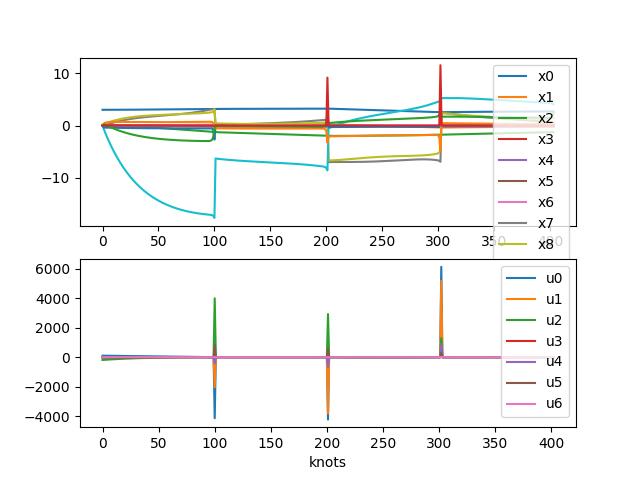
\includegraphics[width=.5\linewidth]{Media/Crocoddyl/ExArm/ArmSolution.png}
\caption{Multi-Point Optimal Control of the Manipulator for reaching four targets. The high-control peaks could be handled by a more advanced solver (e.g. box-ddp), but were not performed here.}
\end{figure}

\subsection{Talos Legs: Bipedal Walking}
The Crocoddyl library offers an example for bipedal walking with the lower body of the Talos \cite{stasse2017talos} Robot. The results of the solved trajectory can be found in Figure \ref{fig:TalosGait}. 

\begin{figure}[h!]
\centering
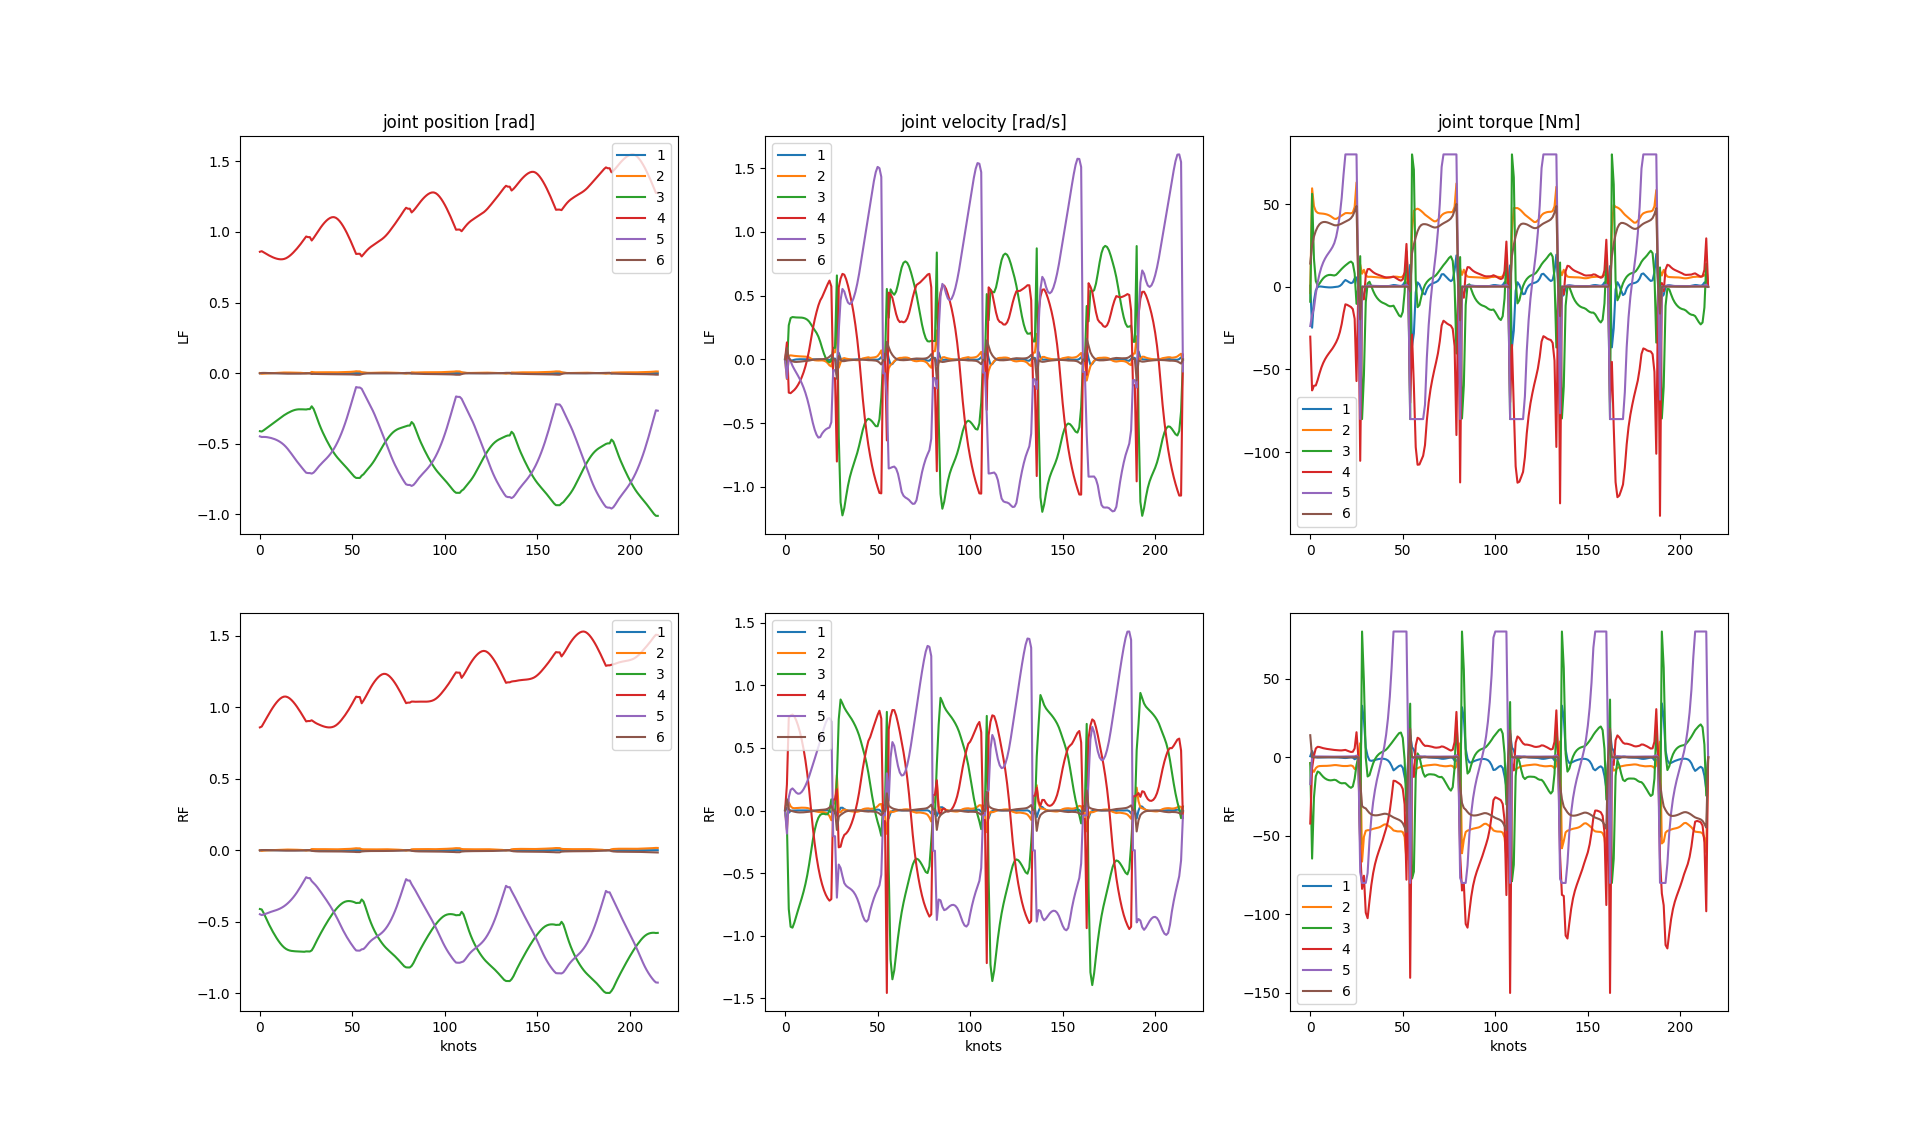
\includegraphics[width=.7\linewidth]{Media/Crocoddyl/ExBiped/TalosGait_Solution.png}
\caption{Results for a walk with three gait-phases.}
\label{fig:TalosGait}
\end{figure}

  



\section{RH5 Results}
Please note once again that all related plots and additional videos can be found in high-quality in the related github repository \cite{julesserOCFrameworks} of this project.
\subsection{Navigating the Files}
The main file for testing RH5 offers several options for setting up, analyzing and constraining the optimization problem of bipedal walking including
\begin{itemize}
\item Choosing a desired URDF 
\item Specifying gait length and variations in step length/height
\item Vary the initial pose of the robot
\item Constraining the torque input (Use different solver)
\item Defining singular or multiple point contacts per foot (Use different class from biped utils)
\end{itemize}

\subsection{Integration of the RH5 Legs into Crocoddyl}
The main issue that had to be solved was related to the underlying URDF file of the robot. In particular: 
\begin{itemize}
\item Choosing one of our several files (abstract-smurf)
\item Cutting out everything apart from the legs and the root joint
\item Fixing the mesh file paths: 

We usually define the path relative to the URDF file location, e.g.
\begin{verbatim}
"../meshes/stl/RH5_Root_Link.001.stl".
\end{verbatim}
The integrated URDF parser in Crocoddyl instead, expects the path specified via the package URI, e.g. 
\begin{verbatim}
"package://abstract-smurf/meshes/stl/RH5_Root_Link.001.stl".
\end{verbatim}
\item Adjust the contact frames for the Walking Problem.
\end{itemize}

\subsection{Performing two Steps}
Results are shown in Figure \ref{fig:rh5_two_steps}.
\begin{figure}[h!]
\centering
\begin{subfigure}{.4\textwidth}
  \centering
  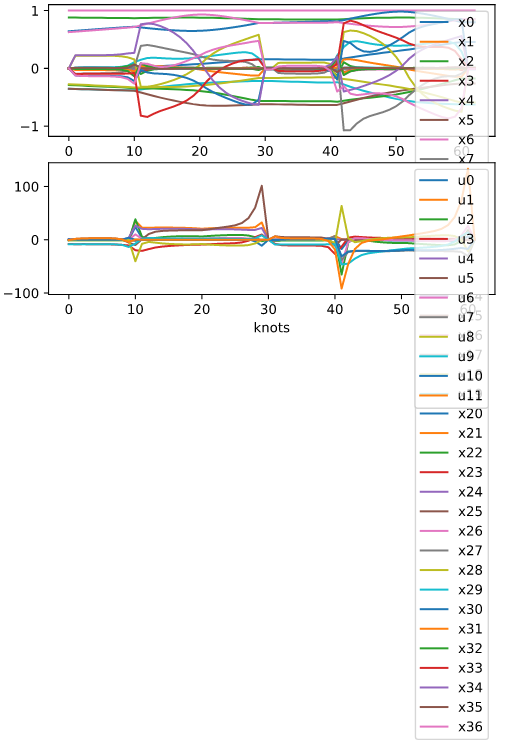
\includegraphics[width=1\linewidth]{Media/Crocoddyl/RH5/2Steps/RH52Steps_Solution.png}
  \caption{Optimal Trajectory and Conrol Inputs}
\end{subfigure}%
\begin{subfigure}{.4\textwidth}
  \centering
  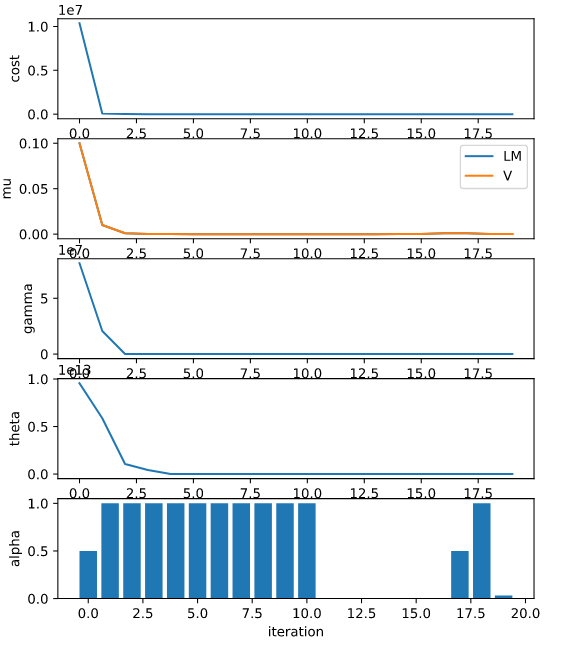
\includegraphics[width=1\linewidth]{Media/Crocoddyl/RH5/2Steps/RH52Steps_Convergence.png}
  \caption{Convergence of Solution}
\end{subfigure}
\caption{Results for a solved shooting problem defining two steps.}
\label{fig:rh5_two_steps}
\centering
\end{figure}

\subsection{Performing a Full Gait}
Results for a full gait (6 consecutive steps) are shown in Figure \ref{fig:rh5_full_gait}.
\begin{figure}[h!]
\centering
\begin{subfigure}{.8\textwidth}
  \centering
  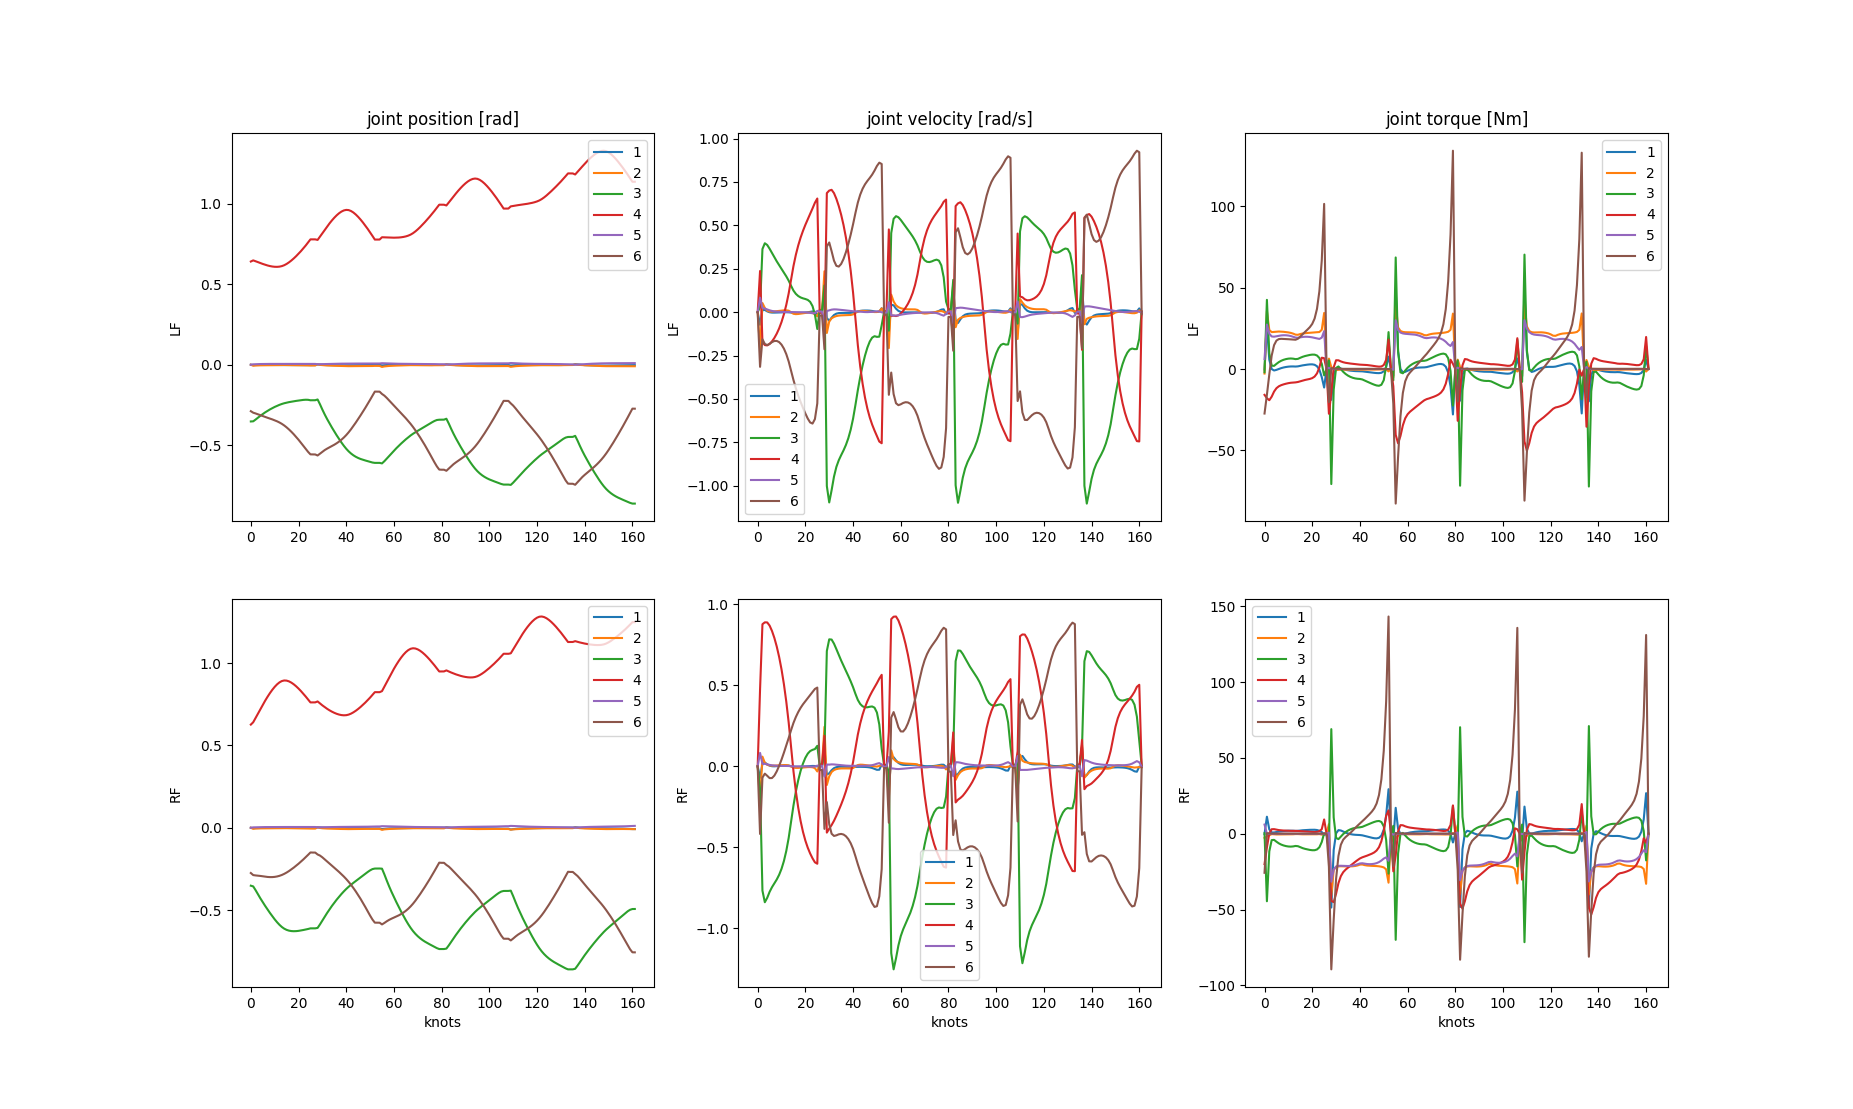
\includegraphics[width=1\linewidth]{Media/Crocoddyl/RH5/RH5Gait_Solution.png}
  \caption{Solution for states and torques.}
\end{subfigure}
\begin{subfigure}{.8\textwidth}
  \centering
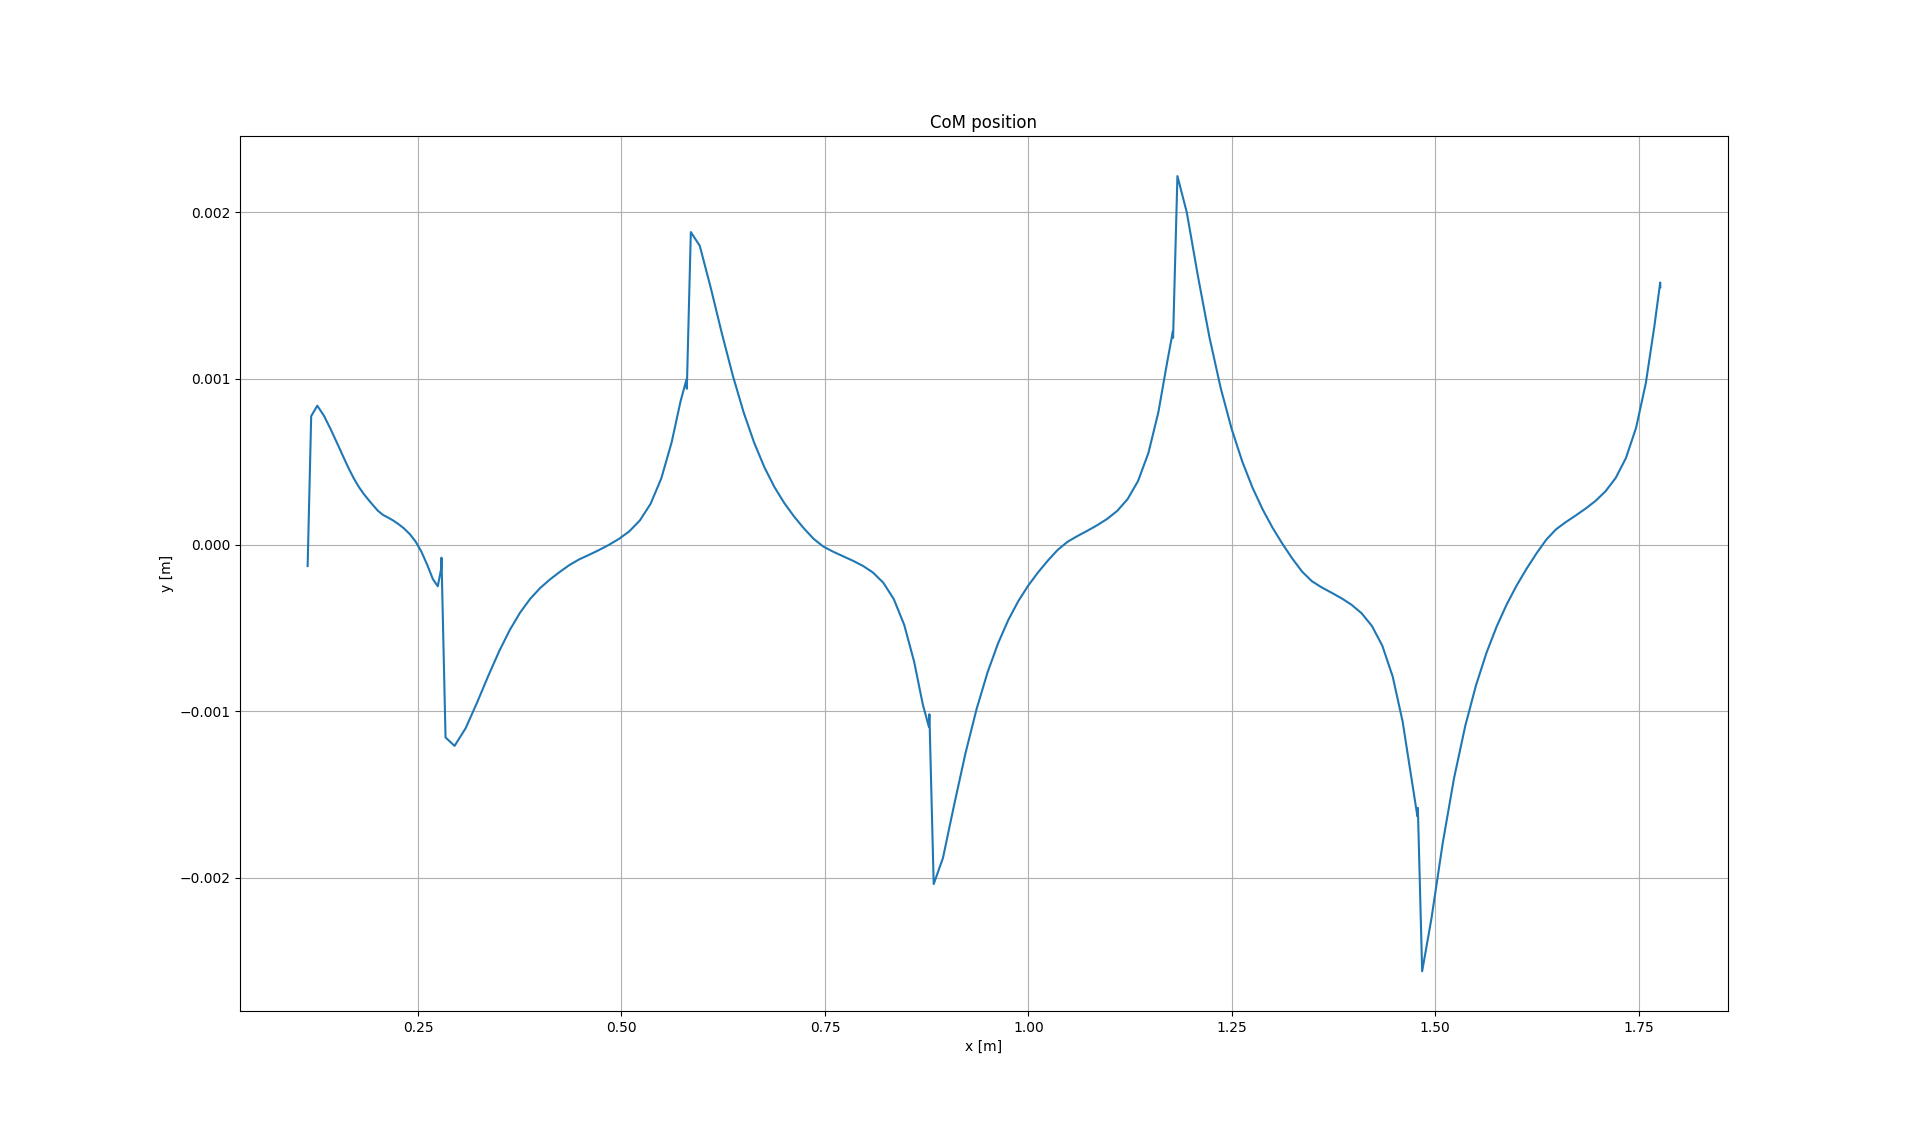
\includegraphics[width=1\linewidth]{Media/Crocoddyl/RH5/RH5Gait_CoM.png}
\caption{CoM results.}
\end{subfigure}
\caption{Results for a walk with three gait-phases. The walk is implemented as a sequence of three  consecutive shooting problems similar to the 2 steps task.}
\label{fig:rh5_full_gait}
\centering
\end{figure}

\subsection{Torque-Constrained Full Gait}
It is possible to constrain the input torques via the limits that are parsed from the URDF. However, the correct solver (box-ddp) needs to be applied to the OC problem for considering these limits.  Results are shown in Figure \ref{fig:rh5_constrain_torque}
\begin{figure}[h!]
\centering
\begin{subfigure}{.8\textwidth}
  \centering
  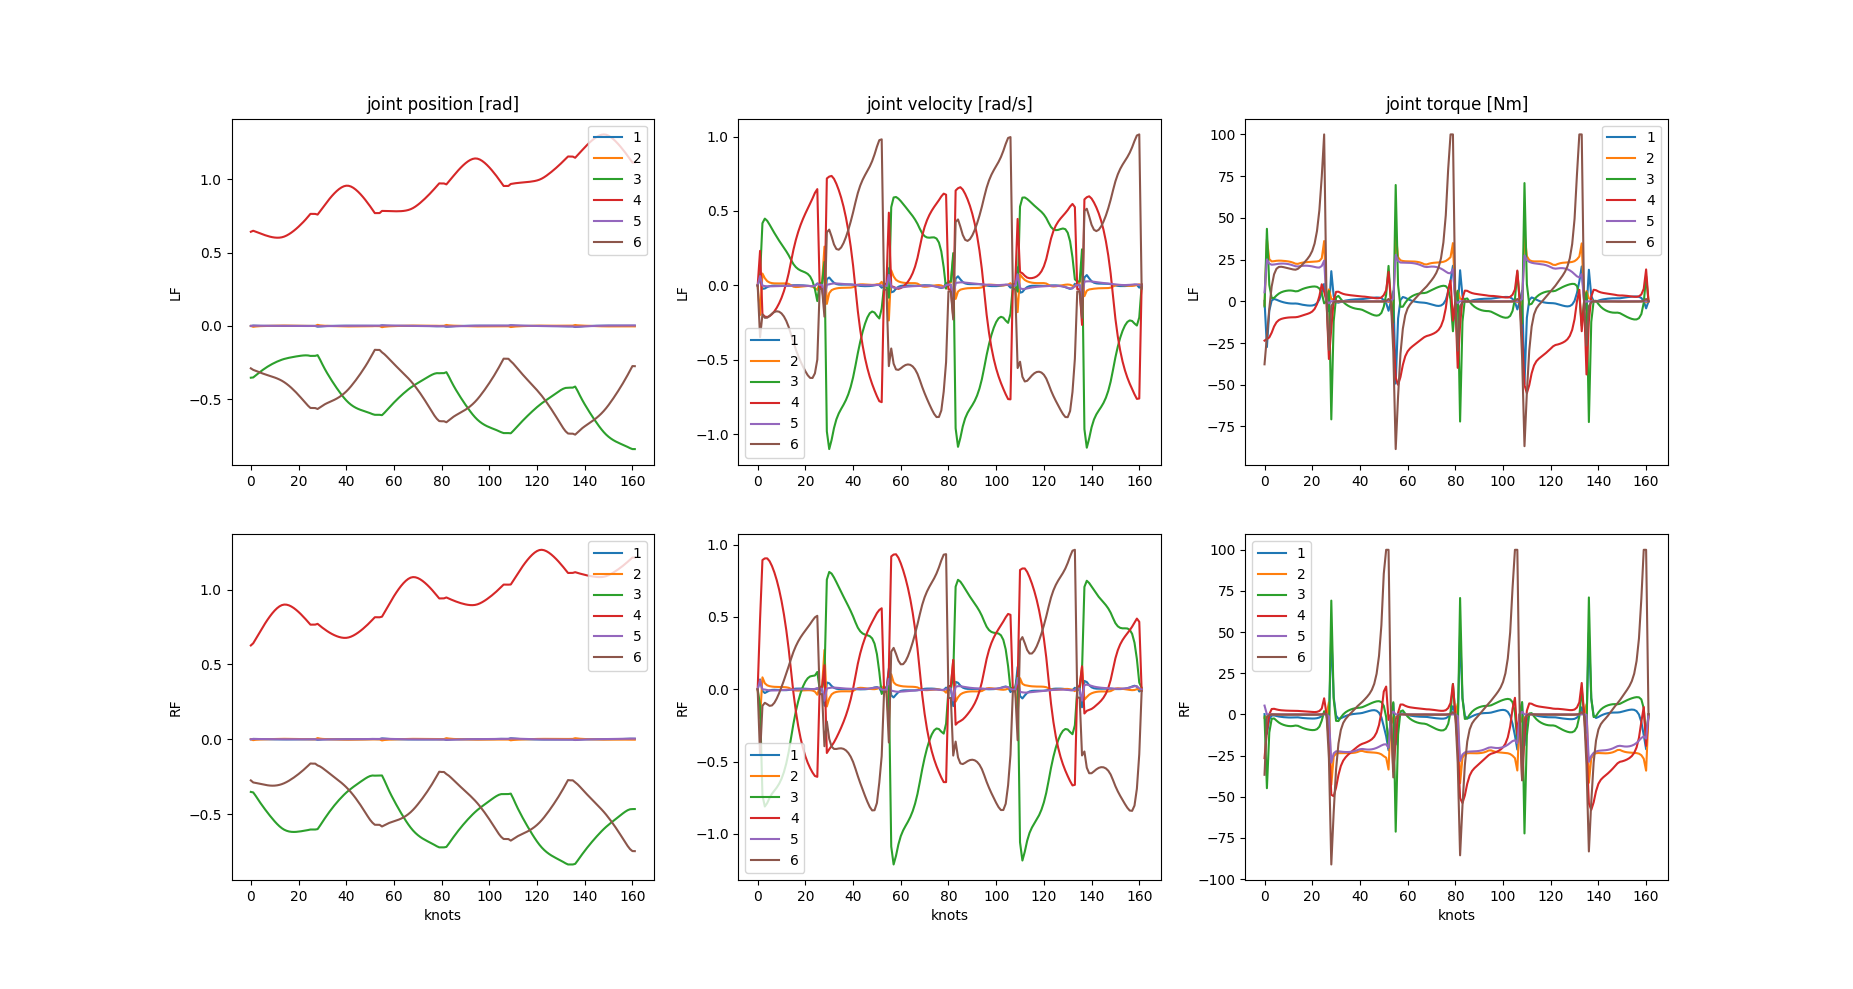
\includegraphics[width=1\linewidth]{Media/Crocoddyl/RH5/RH5GaitUbound50Percent_Solution.png}
  \caption{Solution for states and torques.}
\end{subfigure}
\begin{subfigure}{.8\textwidth}
  \centering
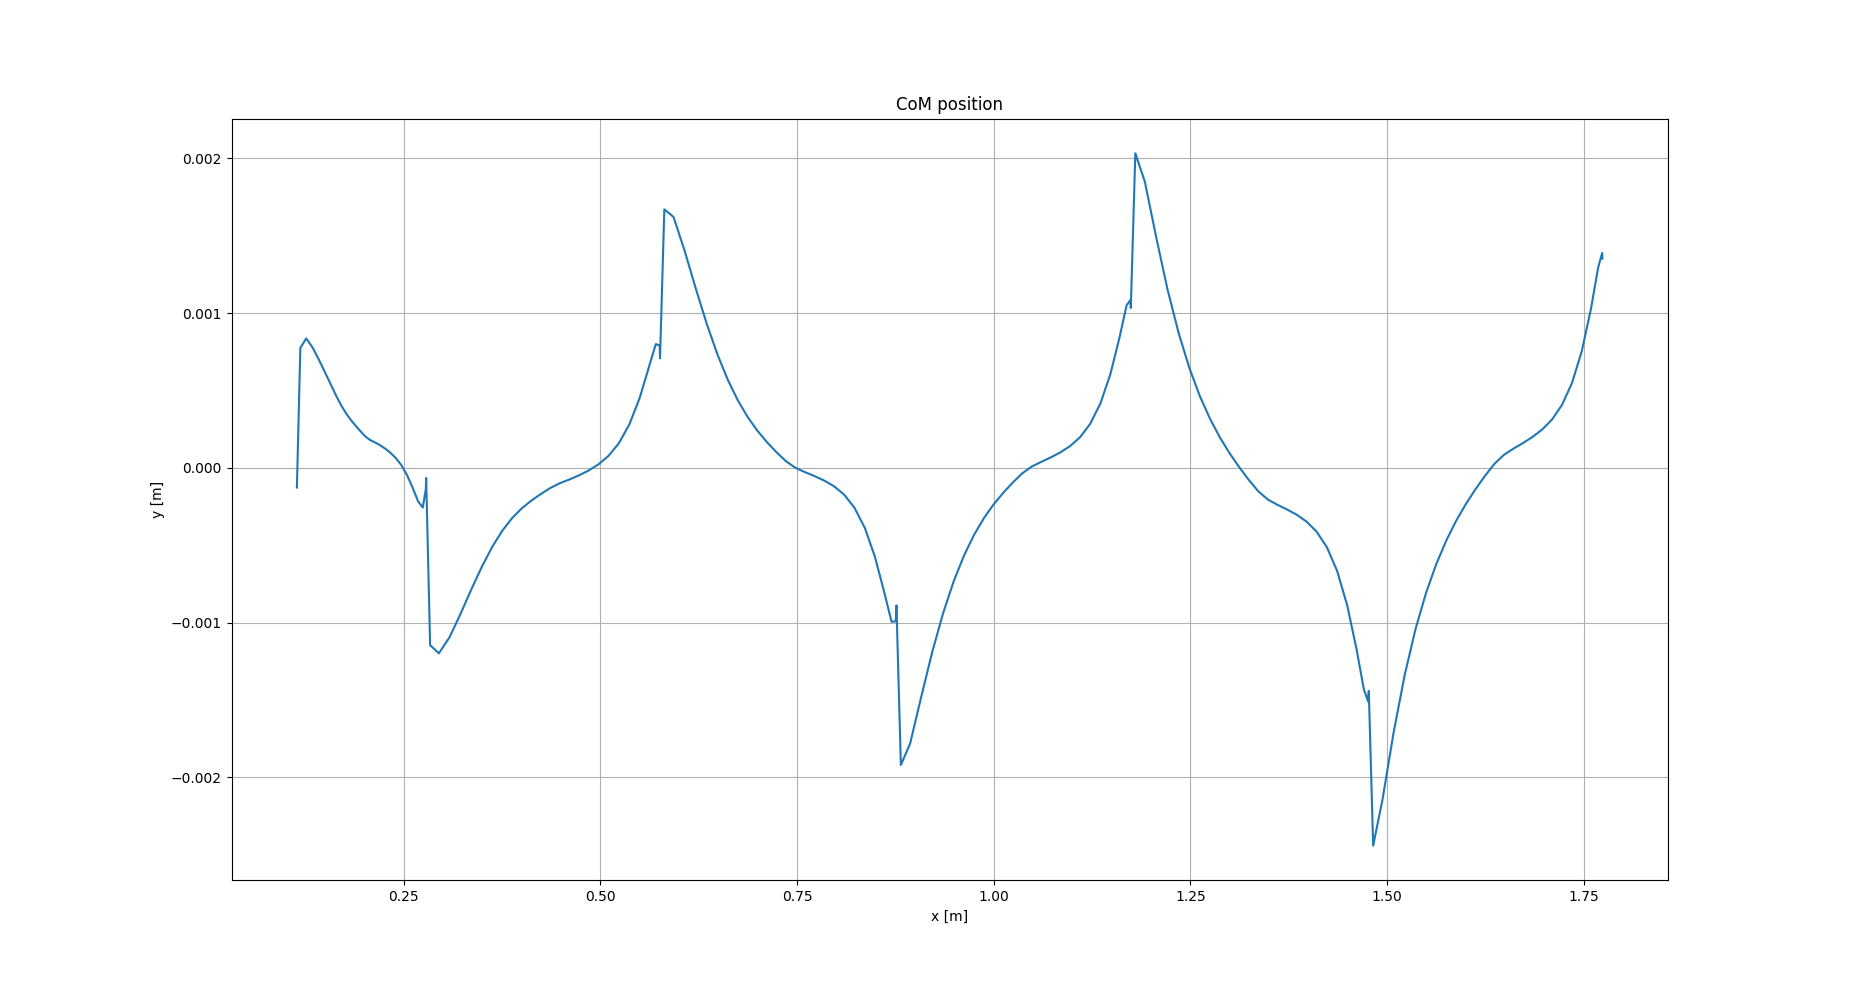
\includegraphics[width=1\linewidth]{Media/Crocoddyl/RH5/RH5GaitUbound50Percent_CoM.png}
\caption{CoM results.}
\end{subfigure}
\caption{Results for full gait with bounded input torques. To be even more restrictive, the available torques form the URDF have been reduced artificially by 50 percent. The effect becomes clear for e.g. the AnkleFT.}
\label{fig:rh5_constrain_torque}
\centering
\end{figure}

\subsection{Initial Pose Variants: Starting Near the Zero Configuration}
The full gait has been initialized according to the pose specifications from the RH5 DFKI smurf file. In this and the following section, two solutions for other initial poses are presented: One near the zero configuration and one at the zero configuration.

\begin{figure}[h!]
\centering
\begin{subfigure}{.8\textwidth}
  \centering
  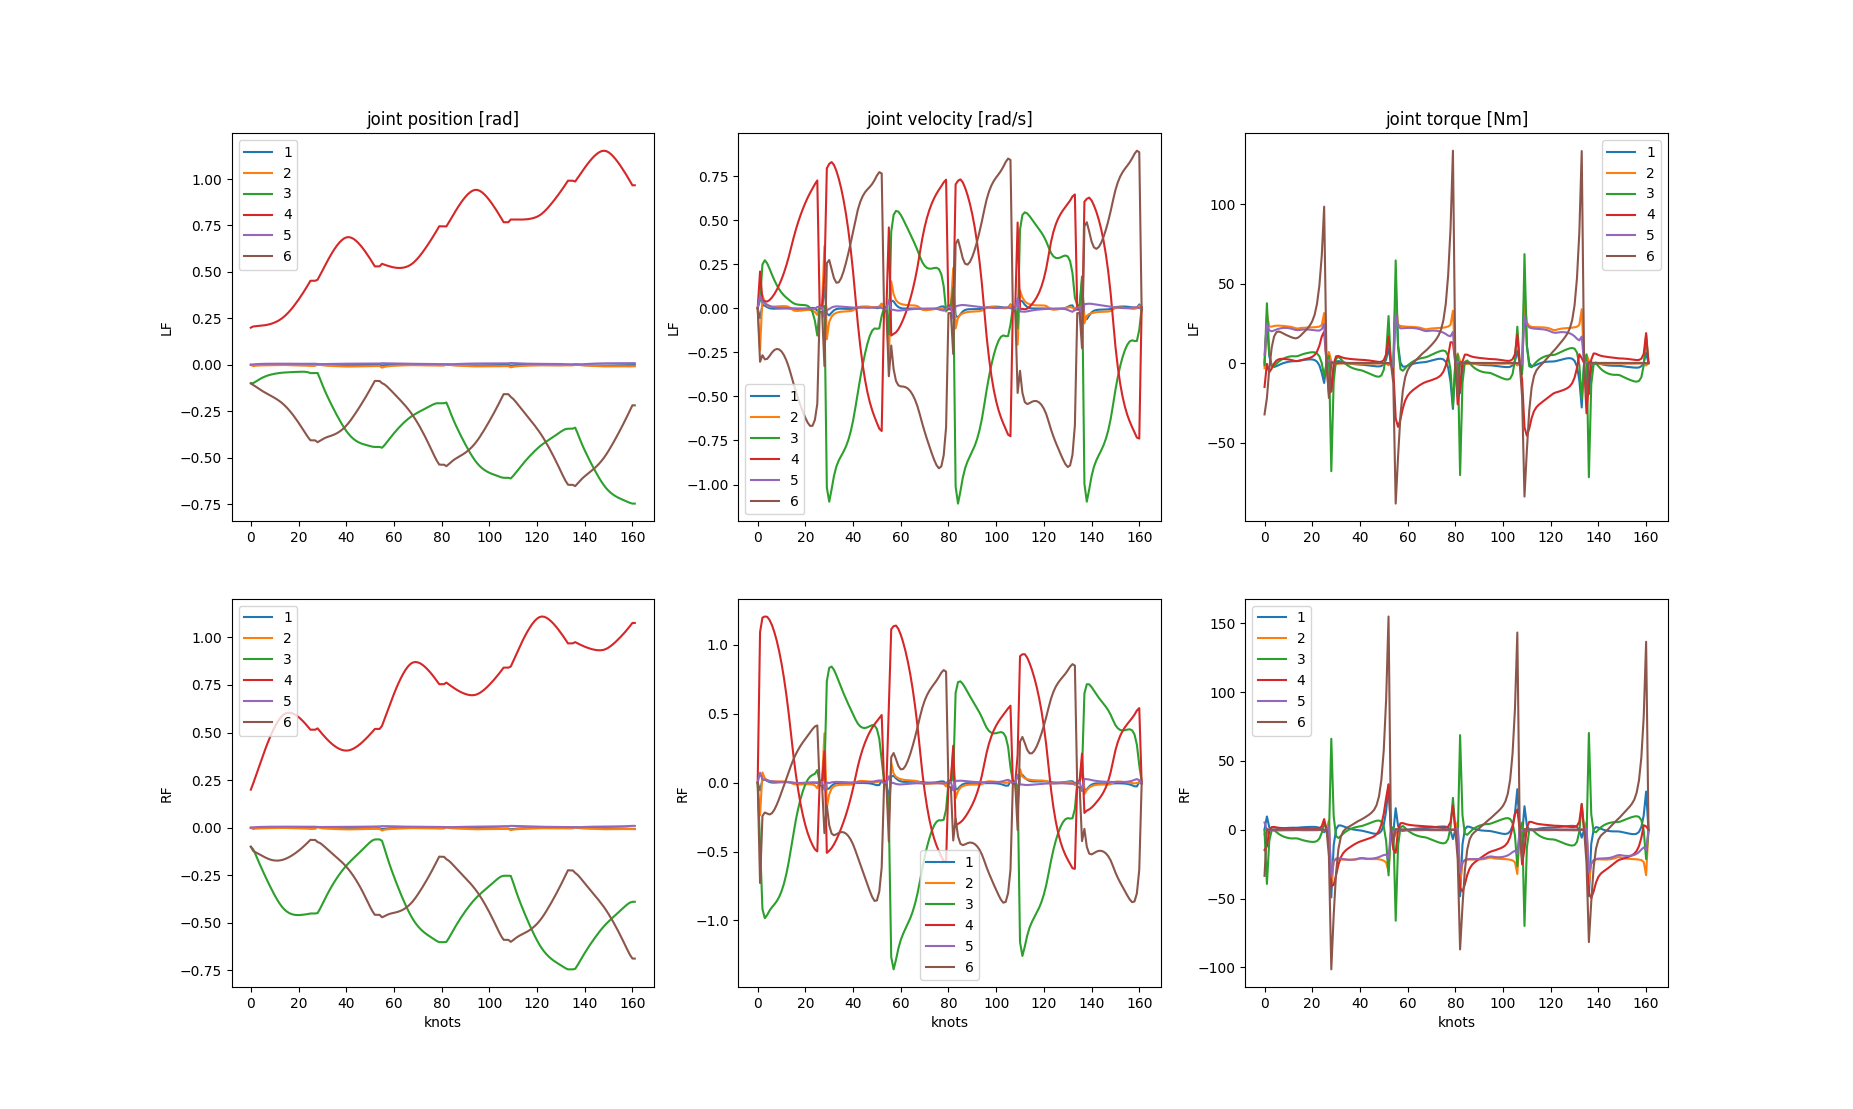
\includegraphics[width=1\linewidth]{Media/Crocoddyl/RH5/InitPoseVariants/RH5GaitInitNearZeroConfig_Solution.png}
  \caption{Solution for states and torques}.
\end{subfigure}
\begin{subfigure}{.8\textwidth}
  \centering
  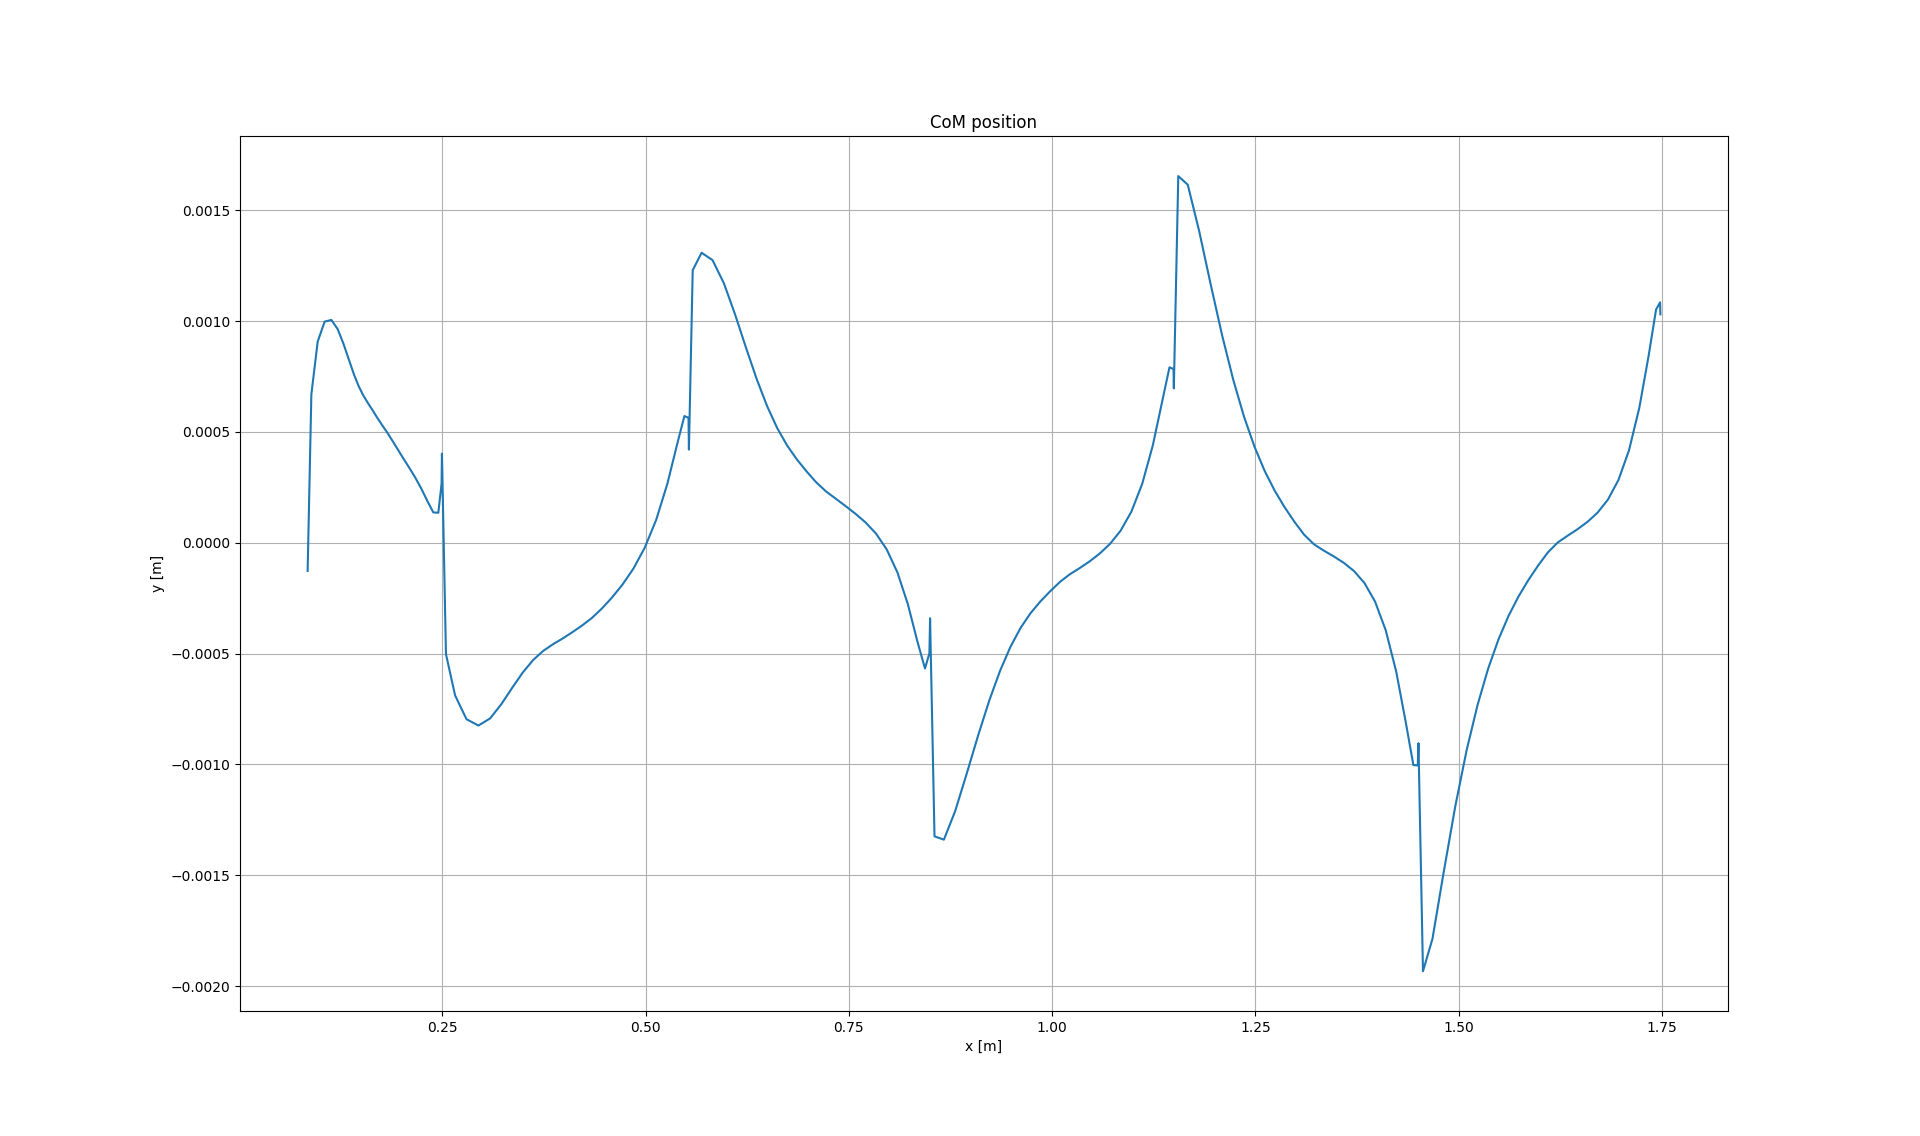
\includegraphics[width=1\linewidth]{Media/Crocoddyl/RH5/InitPoseVariants/RH5GaitInitNearZeroConfig_CoM.png}
\caption{CoM results.}
\end{subfigure}
\caption{Results for the full gait with initial pose \textbf{near} the zero configuration. q0=[0,0,-0.1,0.2,0,-0.1, 0,0,-0.1,0.2,0,-0.1] where  n=12 and represents the joint angles [rad] for the left and right leg.}
\label{fig:rh5_init_near_zero}
\centering
\end{figure}

\subsection{Initial Pose Variants: Starting At the Zero Configuration}
Initializing at the zero configuration turns out to be more critical. Sometimes the solver converges to a feasable solution (Figure \ref{fig:rh5_init_at_zero}), sometimes it does not find a proper solution (Figure \ref{fig:rh5_init_at_zero_failed_solver}).
\begin{figure}[h!]
\centering
\begin{subfigure}{.8\textwidth}
  \centering
  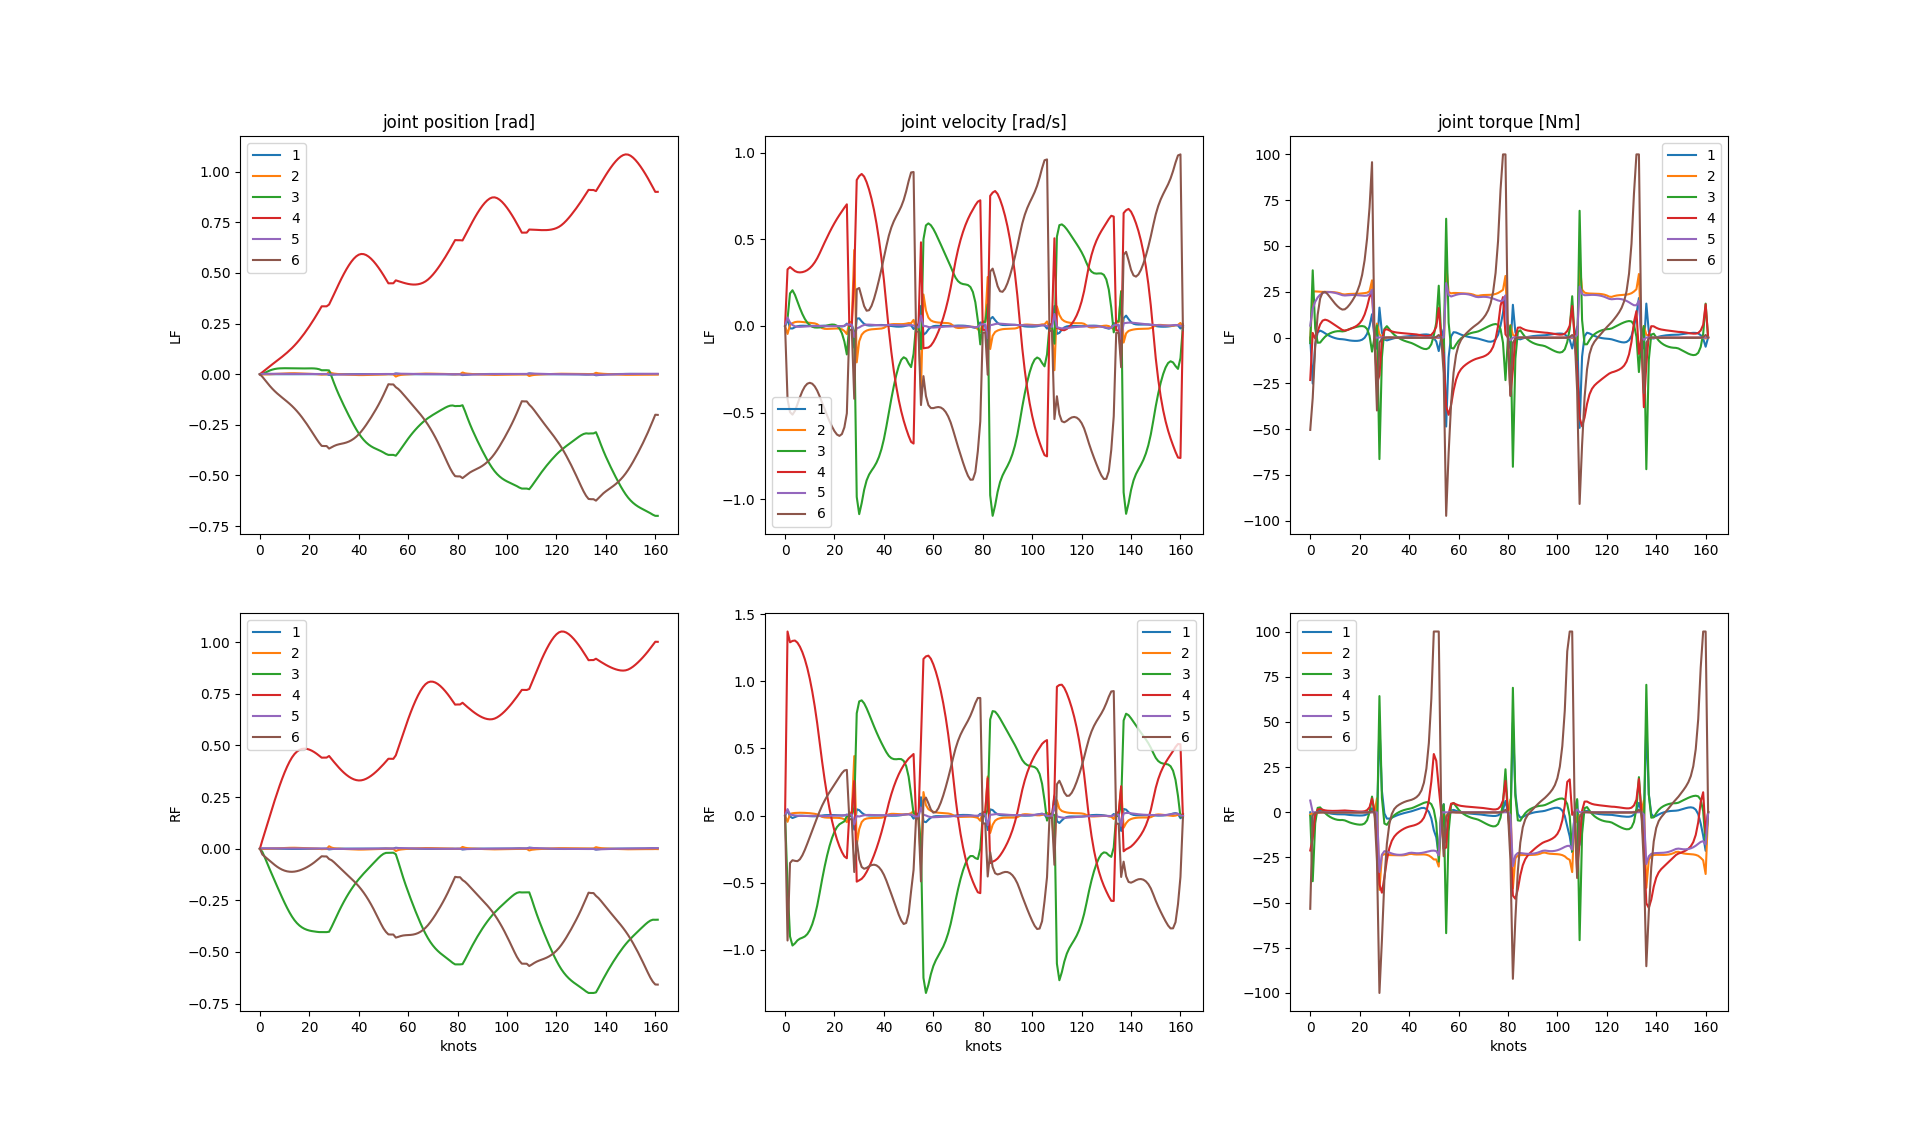
\includegraphics[width=1\linewidth]{Media/Crocoddyl/RH5/InitPoseVariants/RH5GaitInitZeroConfig_Solution.png}
  \caption{Solution for states and torques}.
\end{subfigure}
\begin{subfigure}{.8\textwidth}
  \centering
  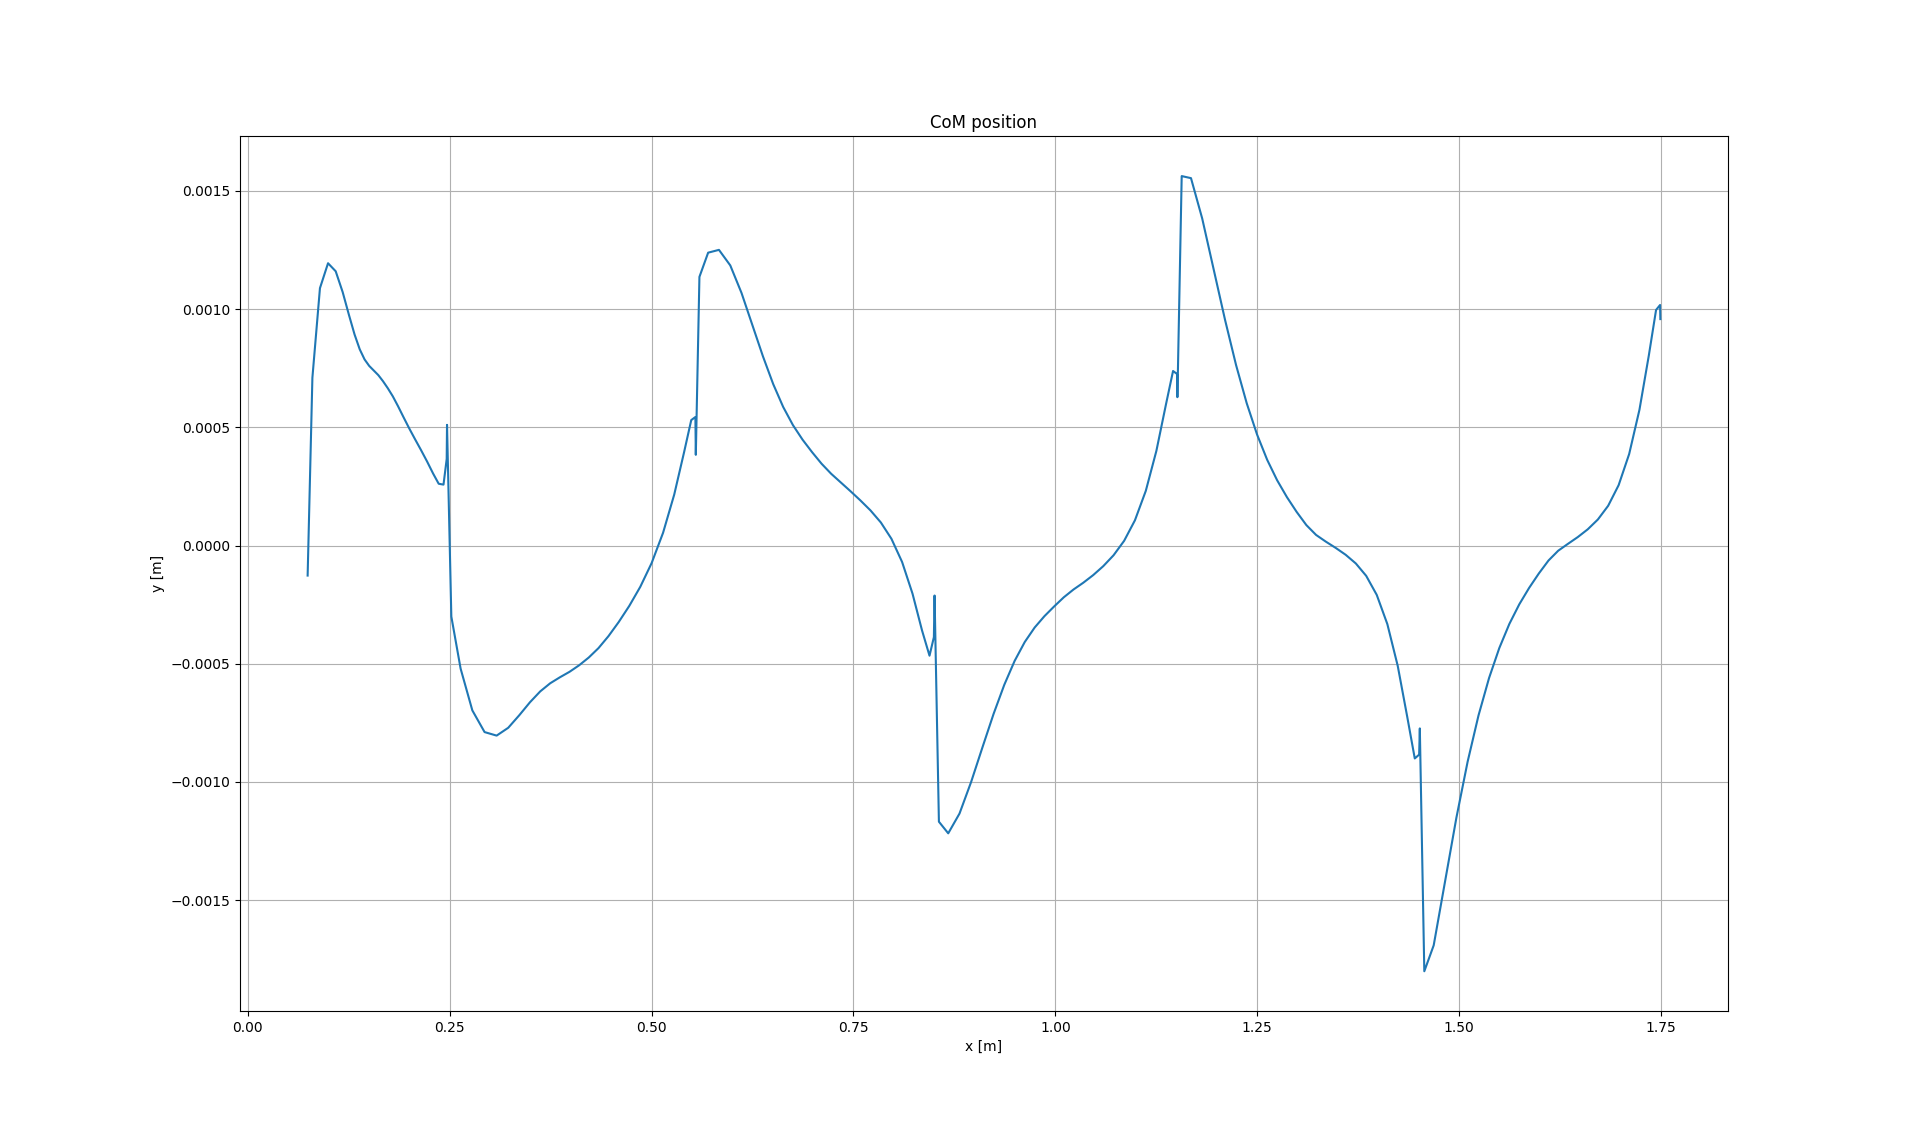
\includegraphics[width=1\linewidth]{Media/Crocoddyl/RH5/InitPoseVariants/RH5GaitInitZeroConfig_CoM.png}
\caption{CoM results.}
\end{subfigure}
\caption{Results for the full gait with initial pose \textbf{at} the zero configuration.}
\label{fig:rh5_init_at_zero}
\centering
\end{figure}

\begin{figure}[h!]
\centering
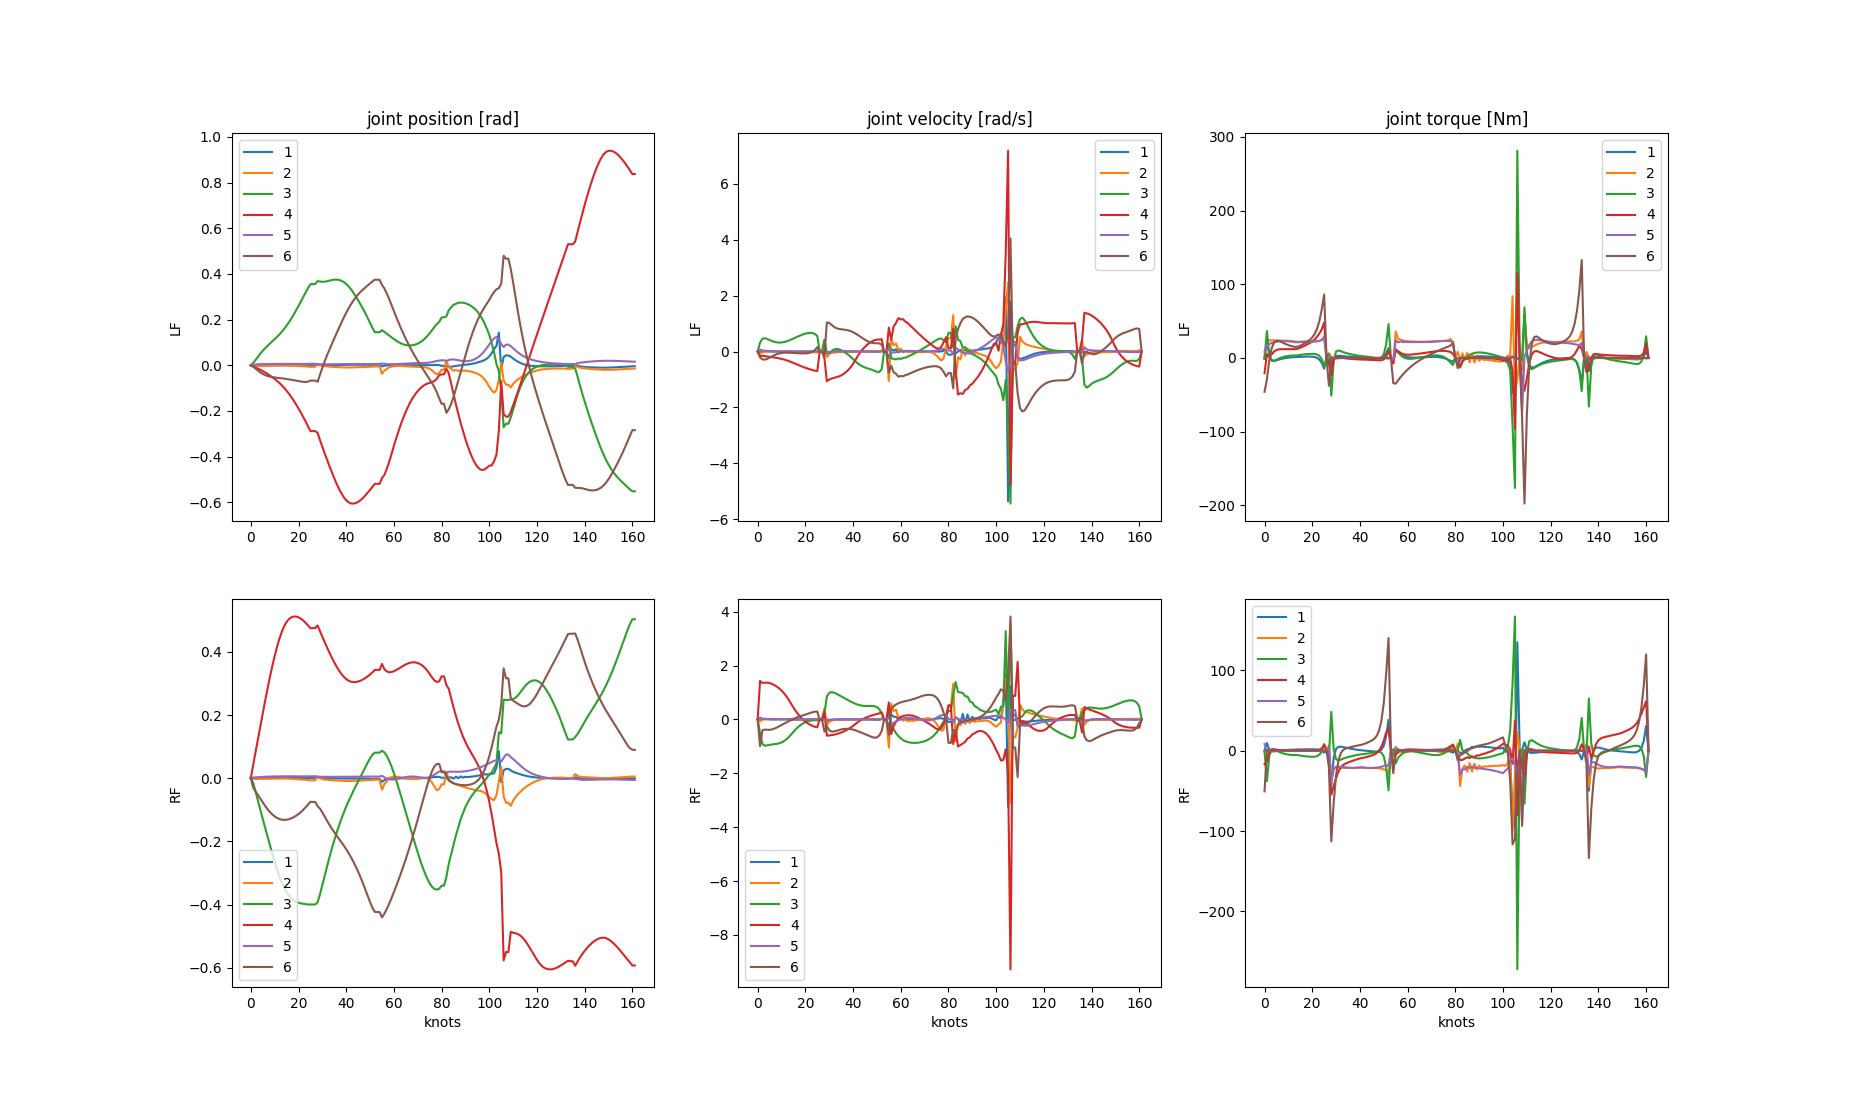
\includegraphics[width=1\linewidth]{Media/Crocoddyl/RH5/InitPoseVariants/RH5GaitInitZeroConfig_Solution_FailedSolver.png}
\caption{Another result for the full gait with initial pose \textbf{at} the zero configuration. The solution appears to be instable and would exceed the torque limits (see video).}
\label{fig:rh5_init_at_zero_failed_solver}
\end{figure}








 